% Author Name: José Areia 
% Author Contact: jose.apareia@gmail.com
% Version: 2.2.7 - 2025-05-23
% Public Repository: https://github.com/joseareia/ipleiria-thesis
% Wiki/Getting Help: https://github.com/joseareia/ipleiria-thesis/wiki

%%% Document Options %%%
\documentclass[
    language=english,
    school=epfl,
    docstage=final,
    media=paper,
    bookprint=false,
    linkcolor=red!80!black,
    chapterstyle=classic,
    coverstyle=classic,
    aiack=true
]{IPLeiriaThesis} % Refer to the Wiki for a list of available options.

%%% Document Version %%%
\DocumentVersion{1.0.0} % Required only if the 'docstage' is set to 'working'.

%%% Document Metadata %%%
% First Author (Mandatory)
\FirstAuthor{Joe Smith}
\FirstAuthorNumber{2230455}

% Second Author (Optional)
% \SecondAuthor{Jane Smith}
% \SecondAuthorNumber{2230456}

% Third Author (Optional)
% \ThirdAuthor{July Smith}
% \ThirdAuthorNumber{2230457}

% Supervisor (Mandatory)
\Supervisor{John Smith}
\SupervisorMail{joe.smith@ipleiria.pt}
% Please provide: [Current Title, Affiliation]
\SupervisorTitle{Full Professor, Polytechnic of Leiria} 

% Co-Supervisor (Optional)
\CoSupervisor{Steve Smith}
\CoSupervisorMail{steve.smith@ipleiria.pt}
\CoSupervisorTitle{Associate Professor, Polytechnic of Leiria}

% Second Co-Supervisor (Optional)
\SecCoSupervisor{Shak Smith}
\SecCoSupervisorMail{shak.smith@ipleiria.pt}
\SecCoSupervisorTitle{Associate Researcher, Computer Science \& Communication Research Centre}

% Title (Mandatory)
\Title{Improving Machine Learning Efficiency Against Noisy Data Sources}

% Subtitle (Mandatory)
\Subtitle{Investigating Advanced Strategies to Mitigate Adverse Effects of Noisy Data}

% University (Mandatory)
\University{Polytechnic of Leiria}

% School (Mandatory)
\School{School of Management and Technology}

% Department (Mandatory)
\Department{Department of Computer Engineering}

% Degree (Mandatory)
\Degree{Master in Cybersecurity \& Digital Forensics}

% Course (Optional)
% \Course{Offensive \& Defensive Cybersecurity}

% Thesis Theme (Mandatory)
\ThesisType{Dissertation/Project/Internship \\ \textcolor{blue}{(Erase the Non-Essential)}}

% Local & Date (Mandatory)
\Date{Leiria, \DTMmonthname{\month} \number\year}

% Academic Year 
\AcademicYear{2024/25}

%%% Loading of Glossary and Acronyms %%%
\makeglossaries
\loadglsentries{Matter/05-Glossary}
\loadglsentries[\acronymtype]{Matter/06-Acronyms}

\begin{document}

%%% Front Matter %%%
\ifthenelse{\equal{\CoverOption}{classic}}{
    \newcommand\BackgroundPicCover{%
    \put(0,0){%
    \parbox[b][\paperheight]{\paperwidth}{%
    \vfill
    \centering
    
\includegraphics[width=\paperwidth,height=\paperheight,keepaspectratio]{Figures/Theme/Cover-BG.pdf}%
    \vfill
    }}}
}{
    \newcommand\BackgroundPicCover{%
    \put(0,0){%
    \parbox[b][\paperheight]{\paperwidth}{%
    \vfill
    \centering
    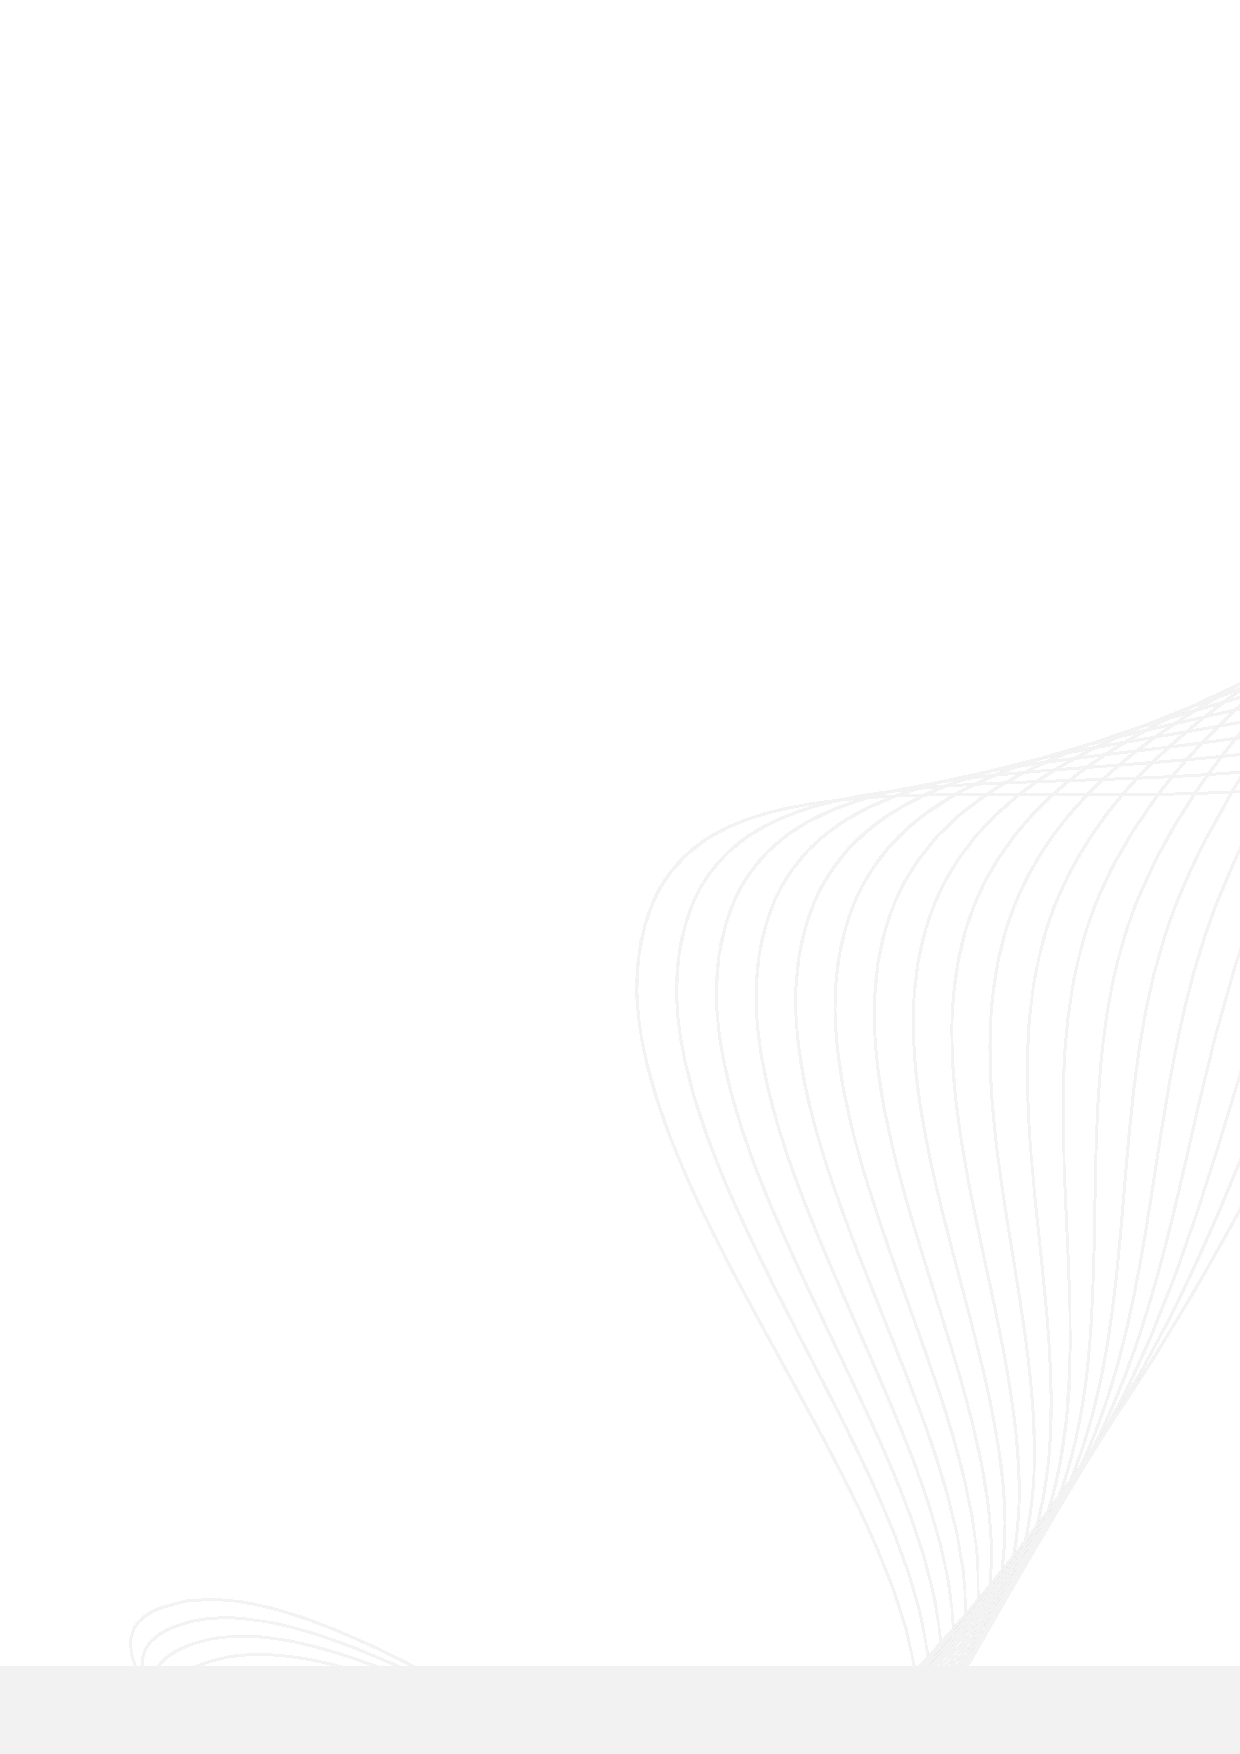
\includegraphics[width=\paperwidth,height=\paperheight,keepaspectratio]{Figures/Theme/Front-Page-BG.pdf}%
    \vfill
    }}}
}

\AddToShipoutPictureBG*{\BackgroundPicCover}

\newgeometry{margin=1.98cm, top=2.15cm, bottom=1.47cm}
\begin{titlepage}
    \latofont
    \ifthenelse{\equal{\CoverOption}{classic}}{\color{white}}{\color{frontpagedark}}
    \vspace*{\baselineskip}

    \ifthenelse{\equal{\CoverOption}{classic}}{
        \ifthenelse{\equal{\SchoolOption}{estg}}{
            \begin{figure}
                
\includegraphics[width=0.485\linewidth]{Figures/Theme/Logotypes/IPLeiria-ESTG-Logo-W.pdf}
            \end{figure}
        }{}
        
        \ifthenelse{\equal{\SchoolOption}{esad}}{
            \begin{figure}
                
\includegraphics[width=0.485\linewidth]{Figures/Theme/Logotypes/IPLeiria-ESAD-Logo-W.pdf}
            \end{figure}
        }{}
        
        \ifthenelse{\equal{\SchoolOption}{esslei}}{
            \begin{figure}
                
\includegraphics[width=0.485\linewidth]{Figures/Theme/Logotypes/IPLeiria-ESSLEI-Logo-W.pdf}
            \end{figure}
        }{}
        
        \ifthenelse{\equal{\SchoolOption}{estm}}{
            \begin{figure}
                
\includegraphics[width=0.485\linewidth]{Figures/Theme/Logotypes/IPLeiria-ESTM-Logo-W.pdf}
            \end{figure}
        }{}
        
        \ifthenelse{\equal{\SchoolOption}{esecs}}{
            \begin{figure}
                
\includegraphics[width=0.485\linewidth]{Figures/Theme/Logotypes/IPLeiria-ESECS-Logo-W.pdf}
            \end{figure}
        }{}
    } {
        \ifthenelse{\equal{\SchoolOption}{estg}}{
            \begin{figure}
                
\includegraphics[width=0.485\linewidth]{Figures/Theme/Logotypes/IPLeiria-ESTG-Logo-B.pdf}
            \end{figure}
        }{}
        
        \ifthenelse{\equal{\SchoolOption}{esad}}{
            \begin{figure}
                
\includegraphics[width=0.485\linewidth]{Figures/Theme/Logotypes/IPLeiria-ESAD-Logo-B.pdf}
            \end{figure}
        }{}
        
        \ifthenelse{\equal{\SchoolOption}{esslei}}{
            \begin{figure}
                
\includegraphics[width=0.485\linewidth]{Figures/Theme/Logotypes/IPLeiria-ESSLEI-Logo-B.pdf}
            \end{figure}
        }{}
        
        \ifthenelse{\equal{\SchoolOption}{estm}}{
            \begin{figure}
                
\includegraphics[width=0.485\linewidth]{Figures/Theme/Logotypes/IPLeiria-ESTM-Logo-B.pdf}
            \end{figure}
        }{}
        
        \ifthenelse{\equal{\SchoolOption}{esecs}}{
            \begin{figure}
                
\includegraphics[width=0.485\linewidth]{Figures/Theme/Logotypes/IPLeiria-ESECS-Logo-B.pdf}
            \end{figure}
        }{}
    }

    \vspace{5.5\baselineskip}

    % Title.
	\noindent
    \makebox[\textwidth][l]{%
        \parbox{\dimexpr\textwidth-4cm\relax}{
            \setstretch{1.03}
            \raggedright\bfseries\fontsize{20}{26}\selectfont\GetTitle
        }
    }

    \vspace{0.8\baselineskip}

    % Subtitle.
    \noindent
    \makebox[\textwidth][l]{%
        \parbox{\dimexpr\textwidth-7cm\relax}{
            \setstretch{1.03}
            \raggedright\fontsize{14}{19}\selectfont\GetSubtitle
        }
    }

    \vspace{35pt}  

    % Author.
    {\noindent\bfseries\fontsize{14}{19}\selectfont\GetFirstAuthor}

    \ifdefined\GetSecondAuthor
        \vspace{8pt}
        {\noindent\bfseries\fontsize{14}{19}\selectfont\GetSecondAuthor}
	\fi

    \ifdefined\GetThirdAuthor
        \vspace{8pt}
        {\noindent\bfseries\fontsize{14}{19}\selectfont\GetThirdAuthor}
	\fi
 
	\vfill

    % School.
	{\noindent\fontsize{10}{12}\selectfont\GetSchool}
	
    % Department.
	{\noindent\fontsize{10}{12}\selectfont\GetDepartment}

    % Degree.
	{\noindent\fontsize{10}{12}\selectfont\GetDegree}

    % Course.
    \ifdefined\GetCourse
        {\noindent\fontsize{10}{12}\selectfont\GetCourse}
	\fi

    \ifthenelse{\equal{\DocStageOption}{working}}{
        \vspace{62pt}
        {\noindent\fontsize{10}{12}\selectfont\overwritecolor{yellow}{\GetDocumentVersion \\ \textit{\today}}} 
        \vspace{62pt}
    }{
        \vspace{125pt}
    }

    % Local & Date.
	{\noindent\fontsize{10}{12}\selectfont\GetDate}

    \vspace{68pt}
\end{titlepage}
\restoregeometry
\MediaOptionLogicBlank
\ifthenelse{\equal{\SchoolOption}{epfl}}{
    \newcommand\BackgroundPicFrontPage{%
        \put(0,0){%
        \parbox[b][\paperheight]{\paperwidth}{%
        \vfill
        \centering
        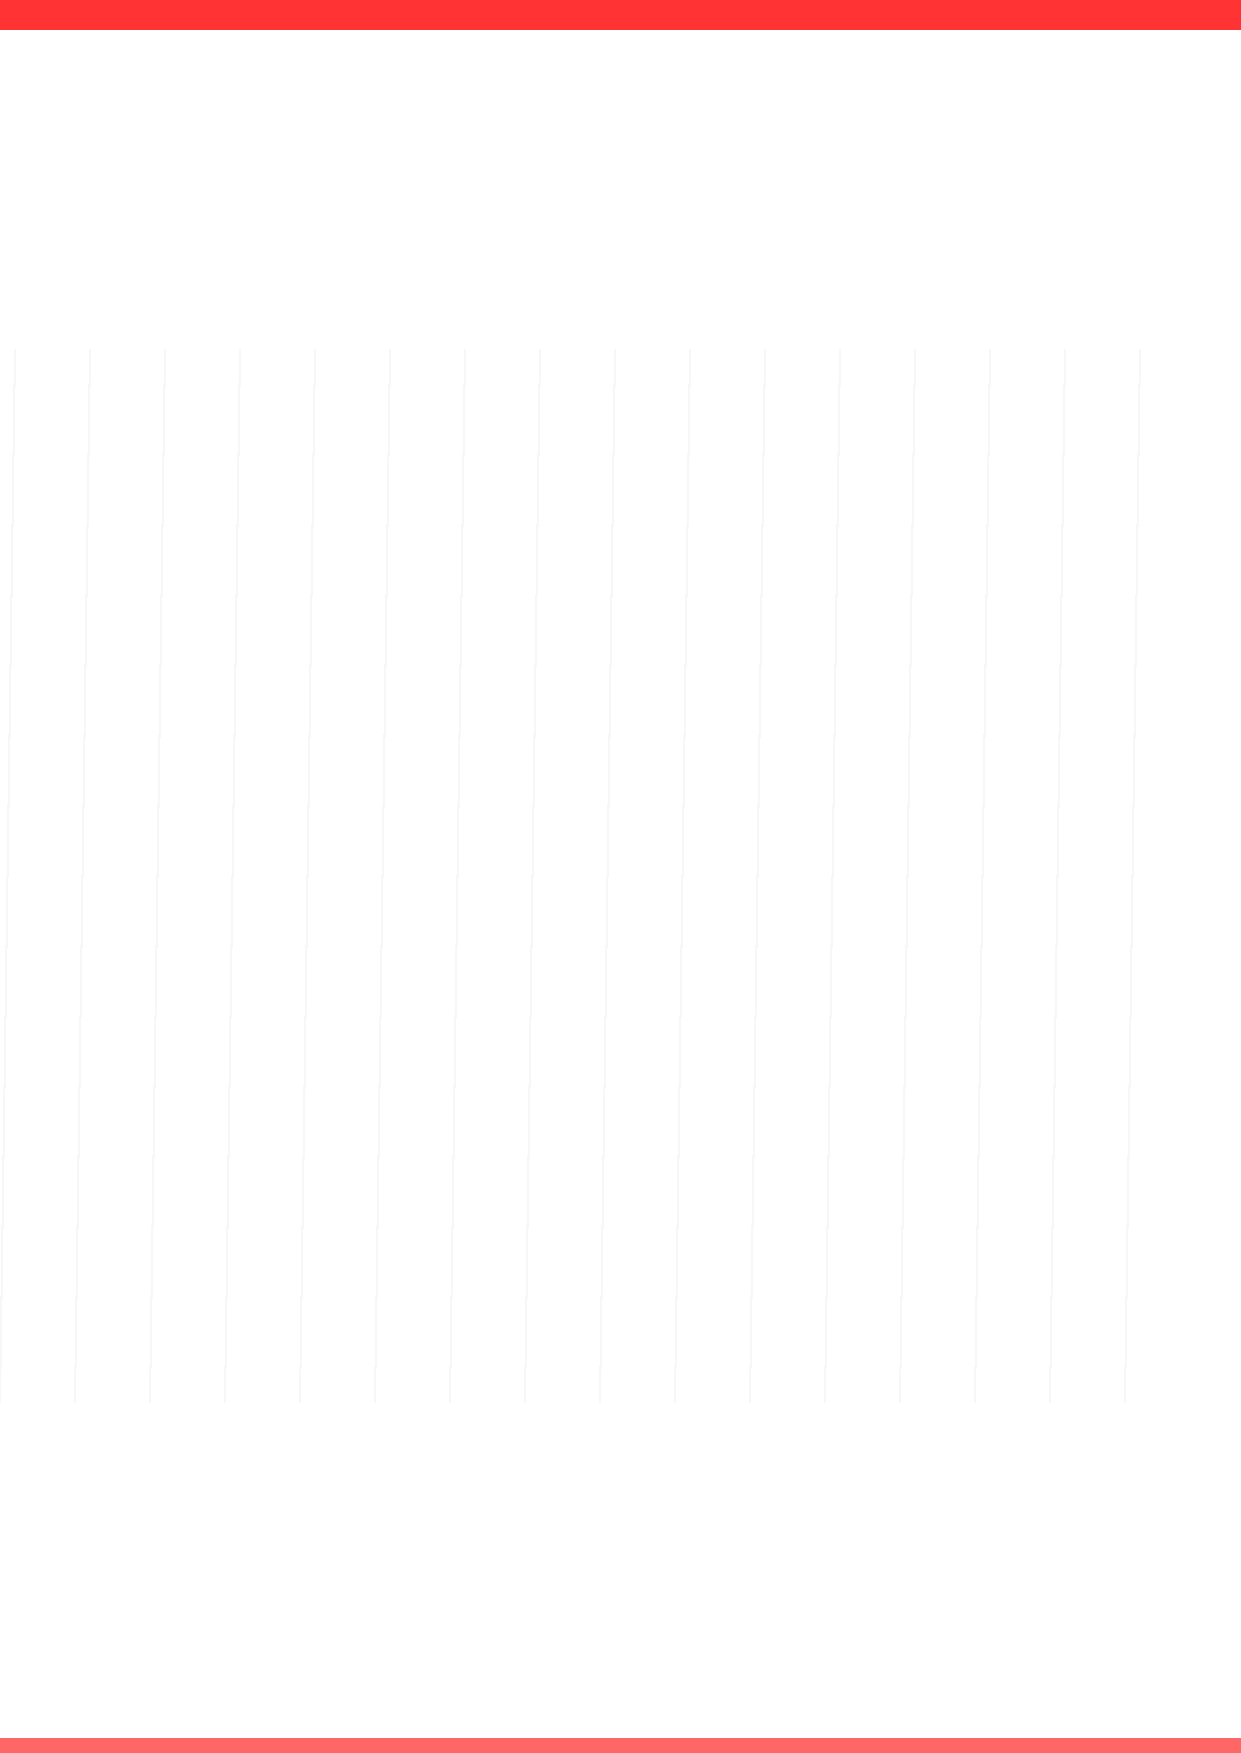
\includegraphics[width=\paperwidth,height=\paperheight,keepaspectratio]{Figures/Theme/EPFL-Front-Page-BG.pdf}%
        \vfill
    }}}
}{
    \newcommand\BackgroundPicFrontPage{%
        \put(0,0){%
        \parbox[b][\paperheight]{\paperwidth}{%
        \vfill
        \centering
        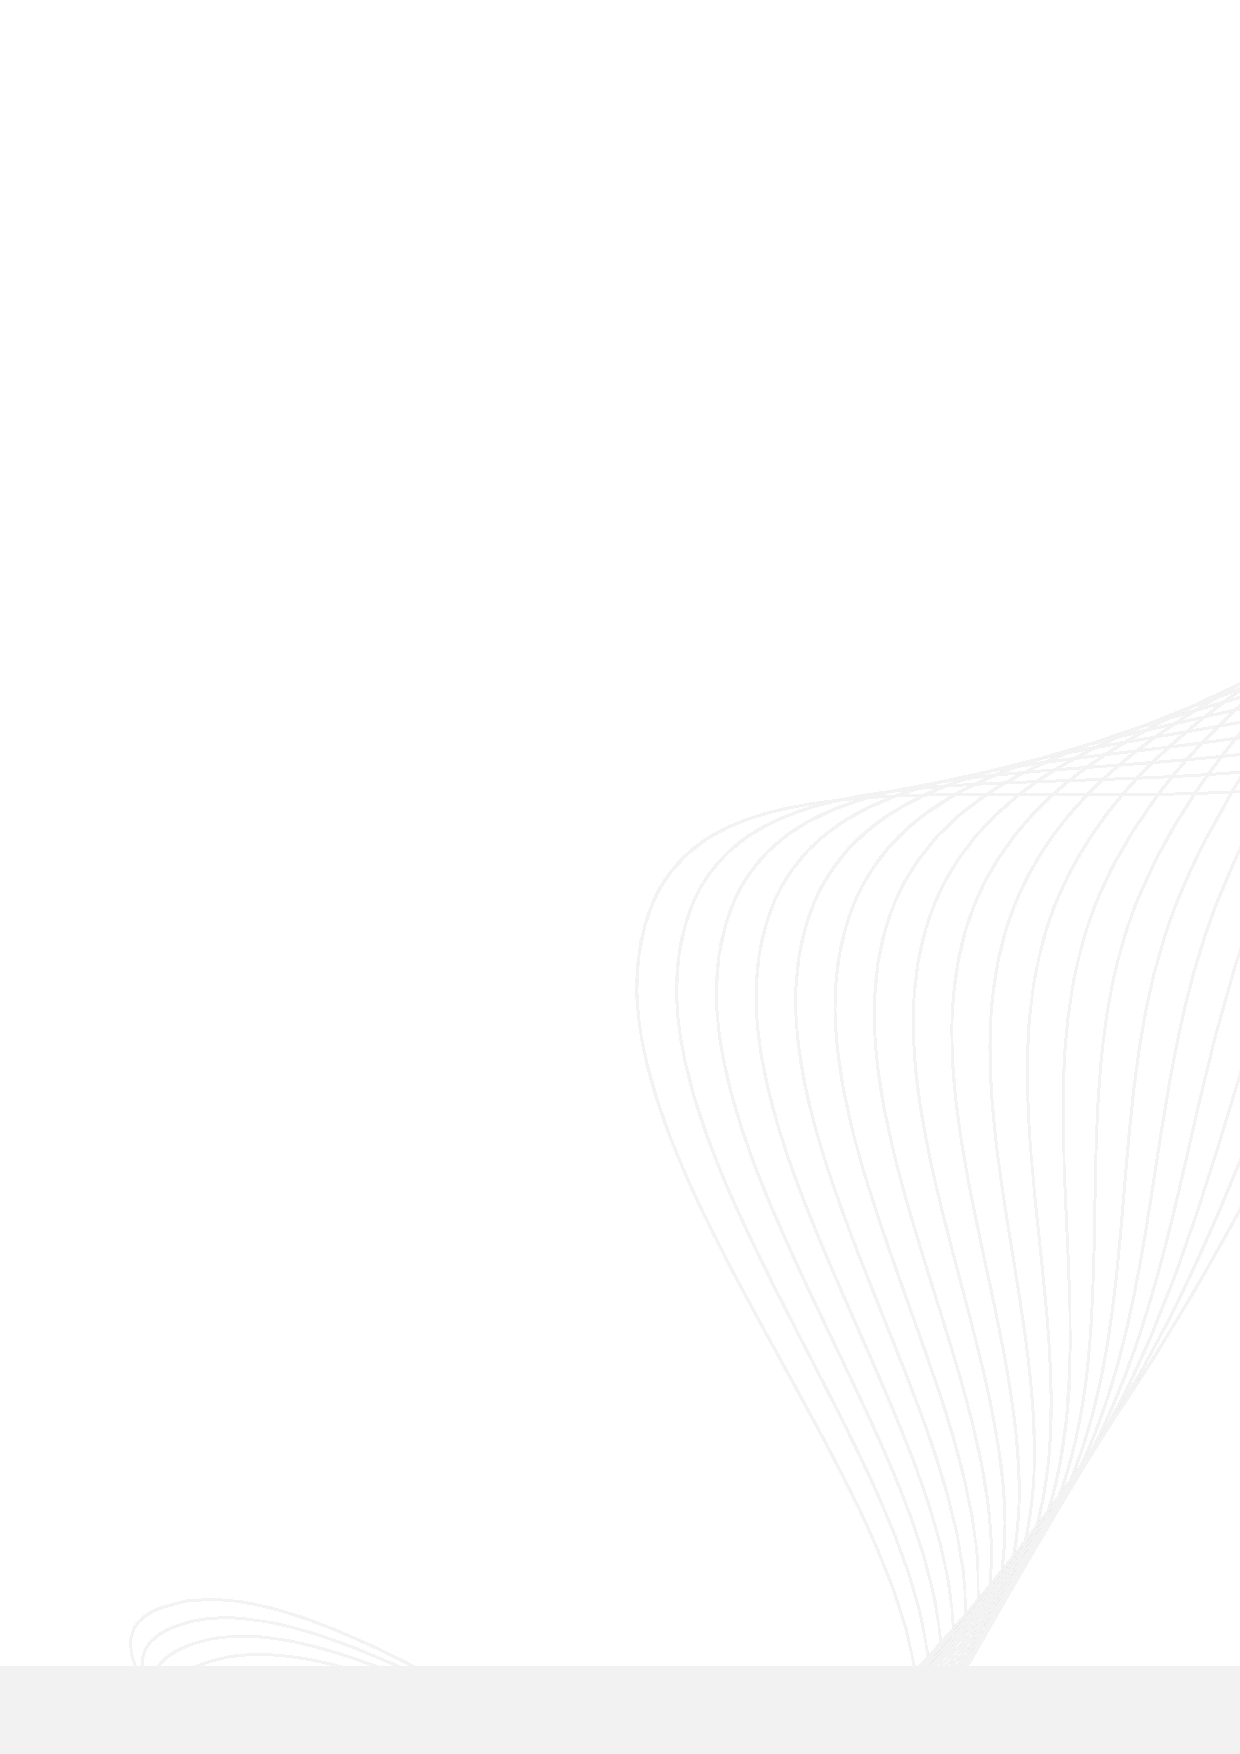
\includegraphics[width=\paperwidth,height=\paperheight,keepaspectratio]{Figures/Theme/Front-Page-BG.pdf}%
        \vfill
    }}}
}
\AddToShipoutPictureBG*{\BackgroundPicFrontPage}

\newgeometry{margin=1.98cm, top=2.15cm, bottom=1.47cm}
\begin{titlepage}
    \latofont
    \color{frontpagedark}
    \vspace*{\baselineskip}

    \ifthenelse{\equal{\SchoolOption}{estg}}{
        \begin{figure}
            
\includegraphics[width=0.485\linewidth]{Figures/Theme/Logotypes/IPLeiria-ESTG-Logo-B.pdf}
        \end{figure}
    }
    
    \ifthenelse{\equal{\SchoolOption}{esad}}{
        \begin{figure}
            
\includegraphics[width=0.485\linewidth]{Figures/Theme/Logotypes/IPLeiria-ESAD-Logo-B.pdf}
        \end{figure}
    }
    
    \ifthenelse{\equal{\SchoolOption}{esslei}}{
        \begin{figure}
            
\includegraphics[width=0.485\linewidth]{Figures/Theme/Logotypes/IPLeiria-ESSLEI-Logo-B.pdf}
        \end{figure}
    }
    
    \ifthenelse{\equal{\SchoolOption}{estm}}{
        \begin{figure}
            
\includegraphics[width=0.485\linewidth]{Figures/Theme/Logotypes/IPLeiria-ESTM-Logo-B.pdf}
        \end{figure}
    }
    
    \ifthenelse{\equal{\SchoolOption}{esecs}}{
        \begin{figure}
            
\includegraphics[width=0.485\linewidth]{Figures/Theme/Logotypes/IPLeiria-ESECS-Logo-B.pdf}
        \end{figure}
    }
    
    \ifthenelse{\equal{\SchoolOption}{epfl}}{
        \begin{figure}
            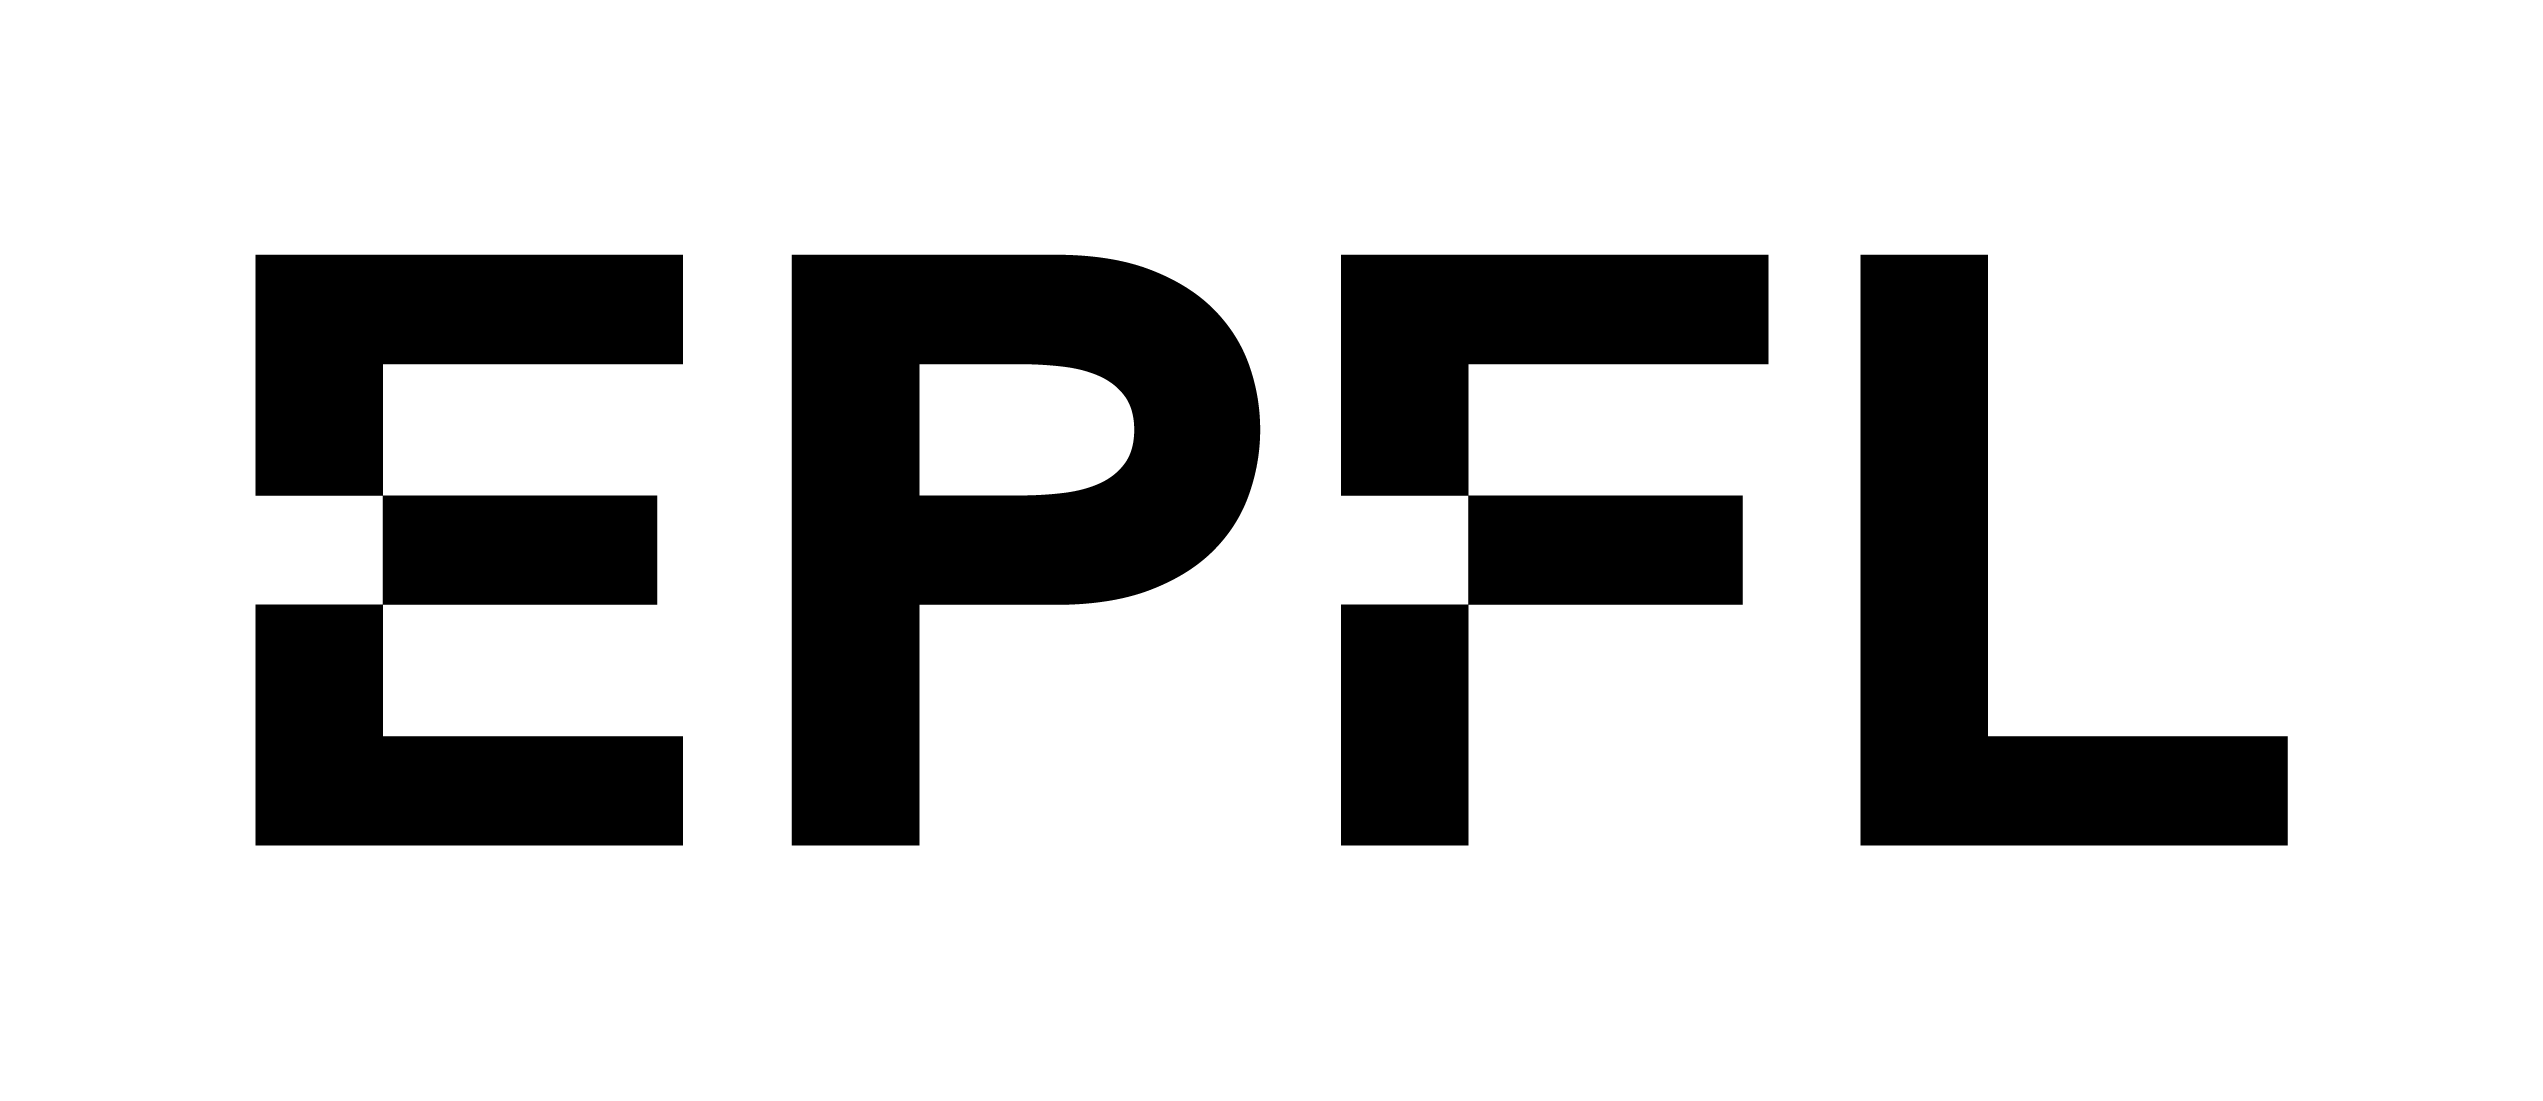
\includegraphics[width=0.485\linewidth]{Figures/Theme/Logotypes/EPFL_Logo_Digital_BLACK_PROD.png}
        \end{figure}
    }

    \vspace{3.5\baselineskip}

    % Title.
	\noindent
    \makebox[\textwidth][l]{%
        \parbox{\dimexpr\textwidth-2.5cm\relax}{
            \setstretch{1.03}
            \raggedright\bfseries\fontsize{20}{26}\selectfont\GetTitle
        }
    }

    \vspace{0.8\baselineskip}

    % Subtitle.
    \noindent
    \makebox[\textwidth][l]{%
        \parbox{\dimexpr\textwidth-7cm\relax}{
            \setstretch{1.03}
            \raggedright\fontsize{14}{19}\selectfont\GetSubtitle
        }
    }

    \vspace{35pt}

    % Author.
    {\noindent\bfseries\fontsize{14}{19}\selectfont\GetFirstAuthor}

    \ifdefined\GetSecondAuthor
        \vspace{8pt}
        {\noindent\bfseries\fontsize{14}{19}\selectfont\GetSecondAuthor}
	\fi

    \ifdefined\GetThirdAuthor
        \vspace{8pt}
        {\noindent\bfseries\fontsize{14}{19}\selectfont\GetThirdAuthor}
	\fi

    \vspace{70pt}    

    {
    \noindent
    \latofont
    \fontsize{10}{12}\selectfont
    \renewcommand{\arraystretch}{0.1}
    \hspace*{-2.5pt}\begin{tabular}{@{}r@{\hspace{5pt}}>{\raggedright\arraybackslash}m{6cm}@{}}
        \textbf{Supervisor:} & \GetSupervisor \\ [-.7ex]
        & \setstretch{0.9}{\fontsize{8}{10}\selectfont\itshape \GetSupervisorTitle} \\ [2ex]
        
        \ifdefined\GetCoSupervisor
            \textbf{Co-supervisor:} & \GetCoSupervisor \\ [-.7ex]
            & \setstretch{0.9}{\fontsize{8}{10}\selectfont\itshape \GetCoSupervisorTitle} \\ [.5ex]
        \fi

        \ifdefined\GetSecCoSupervisor        
            & \GetSecCoSupervisor \\ [-.7ex]
            & \setstretch{0.9}{\fontsize{8}{10}\selectfont\itshape \GetSecCoSupervisorTitle} \\
        \fi
    \end{tabular}
    }
    
    \vfill
	
    % School.
	{\noindent\fontsize{10}{12}\selectfont\GetSchool}
	
    % Department.
	{\noindent\fontsize{10}{12}\selectfont\GetDepartment}

    % Degree.
	{\noindent\fontsize{10}{12}\selectfont\GetDegree}

    % Course.
    \ifdefined\GetCourse
        {\noindent\fontsize{10}{12}\selectfont\GetCourse}
	\fi

    \vspace{45pt}

    % Thesis option.
	{\noindent\fontsize{10}{12}\itshape\selectfont\GetThesisType}

    \vspace{45pt}

    % Local and date.
	{\noindent\fontsize{10}{12}\selectfont\GetDate}

    \vspace{68pt}
\end{titlepage}
\restoregeometry
\MediaOptionLogicBlank

%%% Copyright Statement %%%
\include{Matter/02-Copyright}

%%% Roman Numeration %%%
\pagenumbering{roman}

%%% Acknowledgements %%%
\include{Matter/03-Acknowledgements}

%%% Abstract %%%
\include{Chapters/00-Abstract}

%%% AI Acknowledgement %%%
\include{Matter/04-AI}

%%% Table of Contents, List of Figures and List of Tables %%%
\bookmarktocentry\tableofcontents
\listoffigures
\listoftables

%%% Print: Glossary and Acronyms %%%
\glossarytoc\printnormalglossary
\acronymtoc\printacronymglossary

%%% Arabic Numeration %%%
\pagenumbering{arabic}

%%% Chapters (**Insert Yours Here**) %%%
\include{Chapters/01-Introduction}
\include{Chapters/02-User-Guide}
\include{Chapters/03-Latex-Tutorial}

%%% Bibliography %%%
\renewcommand{\refname}{Bibliography}
\printbibliography[title={\refname},heading=bibintoc]

%%% Appendices: Work that *YOU* Developed %%%
\appendix
\input{Matter/07-Appendices}
\input{Chapters/Appendices/00-AppendixA}
\input{Chapters/Appendices/01-AppendixB}

%%% Annexes: Work that *YOU DID NOT* Develop %%%
\input{Matter/08-Annexes}
\input{Chapters/Annexes/00-AnnexA}

%%% Back Page %%%
\input{Matter/09-Back-Page}

\end{document}